\documentclass[letterpaper,12pt]{article}
\usepackage[letterpaper, portrait, margin=0.5in]{geometry}
\usepackage{graphicx}
\usepackage[utf8]{inputenc}
\usepackage[english]{babel}
\usepackage{fancyhdr}
\usepackage{multicol}
\usepackage[export]{adjustbox}
%Replace svg with students' Scratch ID
\graphicspath{{images/}{svg_images/}}



\begin{document}
\noindent Do not write your name below this line. \\
\noindent \hrule
\begin{center}
{\Large \textbf{\underline{Unit 2: About Me}}}
\end{center}
Scratch Username: JSalac 
 
\noindent \dotfill \\

\noindent The scripts below belong to a sprite named Cat: \\
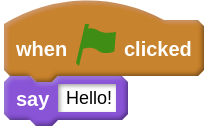
\includegraphics[scale=.4]{q1_script2} \hspace{1cm}
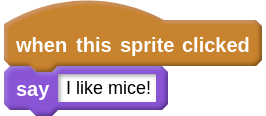
\includegraphics[scale=.4]{q1_script1} \hspace{1cm}
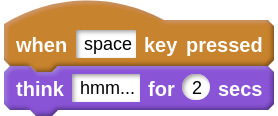
\includegraphics[scale=.4]{q1_script3} \hspace{1cm}
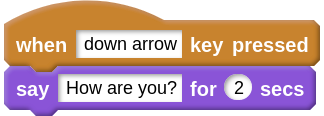
\includegraphics[scale=.4]{q1_script0} \hspace{1cm} \\


\noindent 1. \textbf{Circle}: What should you do to make Cat say "Hello!"?
\renewcommand{\theenumi}{\Alph{enumi}}
\begin{enumerate}
\item Press the space key
\item Click the green flag
\item Press the down arrow
\item Click the sprite
\end{enumerate}

\noindent \dotfill \\

\noindent 2. \textbf{Circle} the Say block that will be run \underline{last}.  \\
\begin{center}
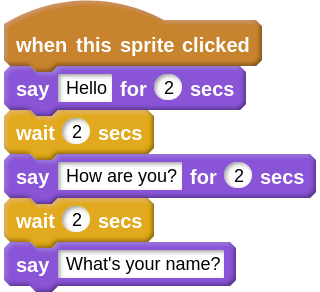
\includegraphics[scale=.4]{q2_script0.png}
\end{center}

\noindent \dotfill \\

\noindent 3. The scripts below belong to a sprite. \textbf{Circle} \underline{all} the scripts that run when you click the sprite. \\

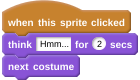
\includegraphics[scale=1,valign=t]{q3_script0.png} \hspace{1cm}
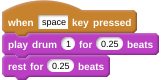
\includegraphics[scale=1,valign=t]{q3_script1.png} \hspace{1cm}
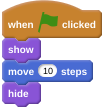
\includegraphics[scale=1,valign=t]{q3_script2.png} \hspace{1cm}
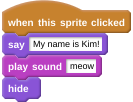
\includegraphics[scale=1,valign=t]{q3_script3.png} \hspace{1cm}


\newpage
\noindent When you click the \textbf{Green Flag}, the stage looks like this:
\begin{center}
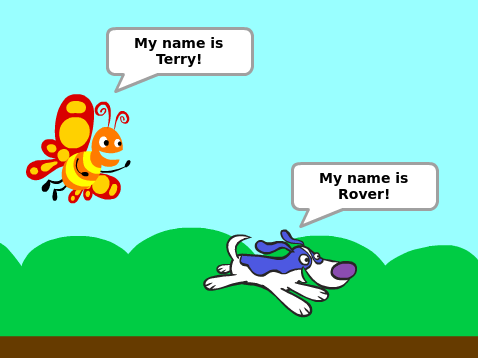
\includegraphics[scale=.5]{q4_stage.png}
\end{center}

\noindent 4a. \textbf{Circle} the script that ran for the butterfly. \\ \\
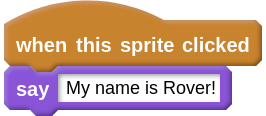
\includegraphics[scale=.4,valign=t]{q4_script0.png} \hspace{1cm}
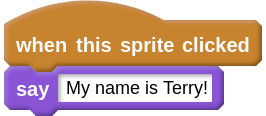
\includegraphics[scale=.4,valign=t]{q4_script1.png} \hspace{1cm}

\includegraphics[scale=.4,valign=t]{q4_script2.png} \hspace{1cm}
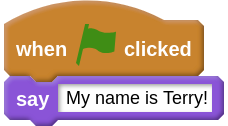
\includegraphics[scale=.4,valign=t]{q4_script3.png} \hspace{1cm}
\vspace{1cm}


\noindent 4b. \textbf{Circle} the script that ran for the dog. \\ \\
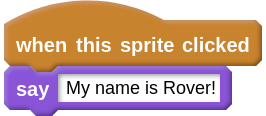
\includegraphics[scale=.4,valign=t]{q4_script0.png} \hspace{1cm}
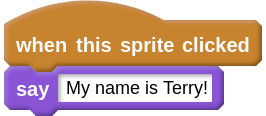
\includegraphics[scale=.4,valign=t]{q4_script1.png} \hspace{1cm}

\includegraphics[scale=.4,valign=t]{q4_script2.png} \hspace{1cm}
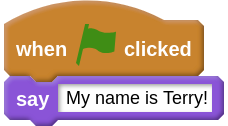
\includegraphics[scale=.4,valign=t]{q4_script3.png} \hspace{1cm}
\vspace{1cm}

\noindent \dotfill

\noindent Compare the two scripts below:
\begin{center}
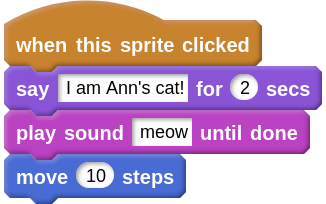
\includegraphics[scale=.4,valign=t]{q5_script0.png} \hspace{0.5in}
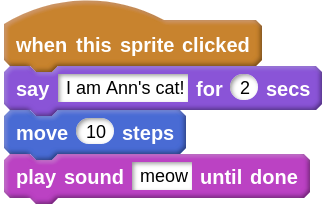
\includegraphics[scale=.4,valign=t]{q5_script1.png}
\end{center}

\noindent 5. \textbf{Circle} what is true:
\renewcommand{\theenumi}{\Alph{enumi}}
\begin{enumerate}
\item They do different actions. 
\item They do the same actions in a different order.
\item There is no difference.
\end{enumerate}
\noindent \dotfill \\

\newpage

\noindent For question 6, please fill in the blanks below. \\ \\
\noindent 6. What will the sprite do when the green flag is clicked?
\begin{center}
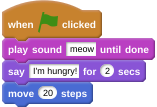
\includegraphics[scale=1]{q6_script0.png}
\end{center}
\noindent First, \hrulefill . \\ \\
Next, \hrulefill . \\ \\

\noindent \dotfill \\

Question 7a and 7b ask about the script below:
\begin{center}
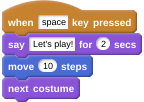
\includegraphics[scale=1]{q7_script0.png}
\end{center}

\noindent 7a. What do you do to make the script run?
\renewcommand{\theenumi}{\Alph{enumi}}
\begin{enumerate}
\item Click the green flag
\item Click the sprite
\item Press the space key \\
\end{enumerate}

\noindent 7b. What does the sprite do when the script runs? \\ \\

\noindent First, \hrulefill . \\ \\
Next, \hrulefill . \\ \\
Last, \hrulefill . \\ \\
\end{document}
